\documentclass[11pt, oneside]{article} 
\usepackage{geometry}
\geometry{letterpaper} 
\usepackage{graphicx}
	
\usepackage{amssymb}
\usepackage{amsmath}
\usepackage{parskip}
\usepackage{color}
\usepackage{hyperref}

\graphicspath{{/Users/telliott_admin/Dropbox/Tex/png/}}
% \begin{center} 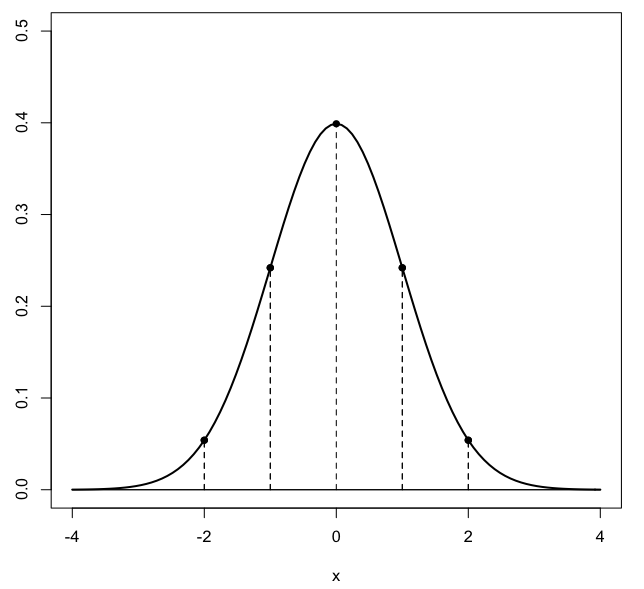
\includegraphics [scale=0.4] {gauss3.png} \end{center}

\title{Numbers}
\date{}

\begin{document}
\maketitle
\Large
This chapter is a bit of a digression, and can easily be skipped, but it's fun and not too technical.

Our ideas about sets of numbers start with the counting numbers or positive integers
\[ 1, 2, 3 \dots \]
which is also known as the set of \emph{natural} numbers, $\mathbb{N}$.

$\mathbb{N}$ is an infinite set.  

Proof by contradiction:  assume there is a greatest natural number.  Add $1$ to it.  

$\square$

We extend $\mathbb{N}$ with the number $0$, also known as the additive identity, plus the negatives or additive inverses of all the numbers in $\mathbb{N}$ where $n + (-n) = 0$:
\[ \mathbb{Z} = \{ \dots - 3, -2, -1 , 0 , 1, 2, 3 \dots \} \]

$\mathbb{Z}$ is what they call a \emph{ring}.  The standard operations addition, subtraction and multiplication are defined and allowed, but not division. The allowed operations always give numbers as results which are contained in $\mathbb{Z}$.

Suppose we want division.  We define the rational numbers $\mathbb{Q}$:
\[ \mathbb{Q} = \frac{p}{q}, \ \ \ \  p \in \mathbb{Z}, q \in \mathbb{N} \]

The rational numbers have great properties.  For example

$\circ$  For any two rational numbers one can find another such number which lies between them.  Here is one possible approach:
\[ r = \frac{1}{2} \ [ \ \frac{p_1}{q_1} +  \frac{p_2}{q_2} \ ] \]

$r$ is a rational number and it lies between the two numbers we started since it is the average of the two.  

Proof:  relabel $s = p_1/q_1$ and $t = p_2/q_2$ thus
\[ r = \frac{1}{2} \ [ s + t \ ] \]
\[ 2r = s + t \]
\[ 2r - 2s = t - s \]
suppose $s < t$, then $t - s > 0$ and so
\[ r - s > 0 \]
\[ r  > s \]
A similar argument will show that
\[ r < t \]
thus
\[ s < r < t \]
$\square$
  
Thus, it is not unreasonable to have the idea that the number line can be divided into pieces as small as you like by finding rational numbers between rational numbers between rational numbers, and so on.

It sounds good, but there is a big problem which you probably know:  some numbers cannot be expressed as the ratio of two integers, for example, $\sqrt{2}$.

Further, $\sqrt{3}$, $\sqrt{5}$, $\sqrt{7}$, etc..  And don't forget $\pi$ and $e$.  Here is a proof that $\sqrt{2}$ is irrational

\begin{center} 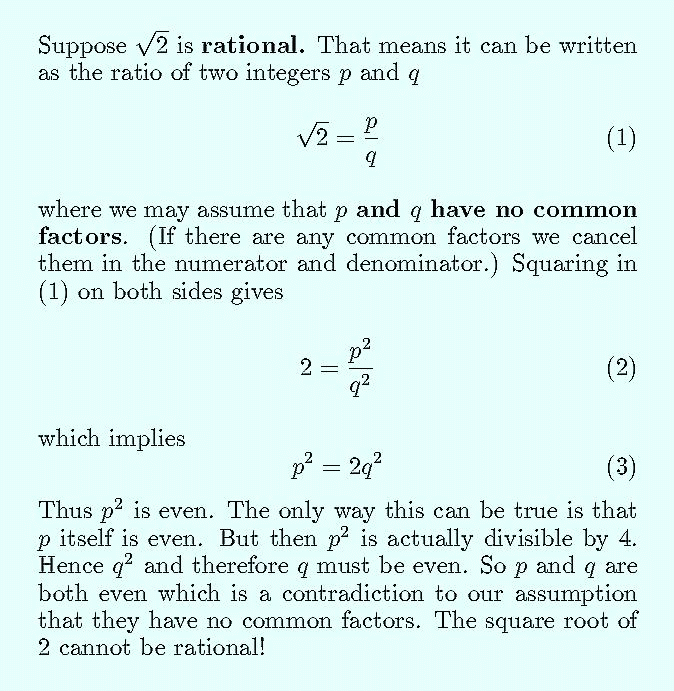
\includegraphics [scale=0.5] {q1.png} \end{center}

To quote Hardy (\emph{A Mathematician's Apology}):

\begin{quote}
The proof is by reductio ad absurdum, and reductio ad absurdum, which Euclid loved so much, is one of a mathematician’s finest weapons. It is a far finer gambit than any chess gambit: a chess player may offer the sacrifice of a pawn or even a piece, but a mathematician offers the game.
\end{quote}

The numbers like $\sqrt{2}$ are said to be \emph{irrational} numbers and the set of these, plus all the other numbers is called the real numbers $\mathbb{R}$.

This led Dedekind to formulate the famous Dedekind cut.  Visualize the standard number line as an infinite line on (an infinite) piece of paper.  

\begin{center} 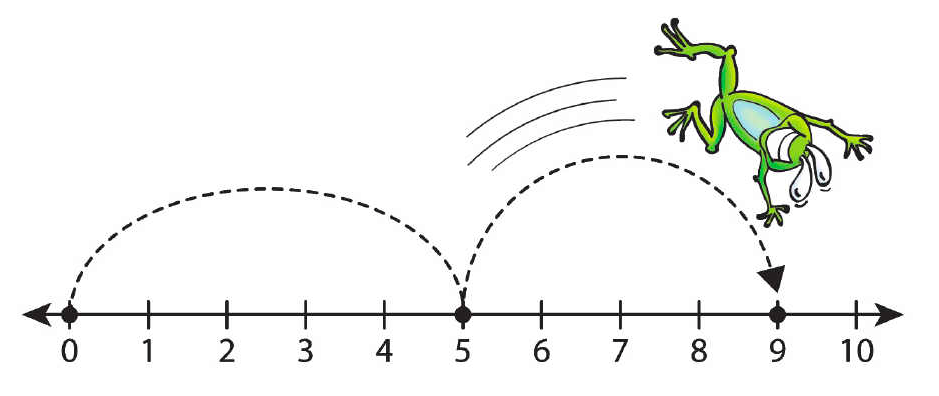
\includegraphics [scale=0.4] {number_line.png} \end{center}

Each real number corresponds to a cut, a knife-edge coming down somewhere on this number line.  Every other number that is not equal to this one, is either $>$ or $<$ the number specified by the cut.

One position is $\sqrt{2}$, one is $7/4$ and so on.

We said that for any two rational numbers one can find a rational number which lies between them.

Three related statements are also true.  We will show that

$\circ$ for any two rational numbers one can find a real number which lies between them

$\circ$ for any two real numbers one can find a rational number which lies between them

$\circ$ for any two real numbers one can find a real number which lies between them

\subsection*{continuum}

$\circ$  Between any two \emph{real} numbers it is always possible to find a rational number.  

Proof:  pick
\[ N \in \mathbb{N} \text{ such that } N > \frac{1}{b-a} \]
Then 
\[ \frac{1}{N} < b - a \]
Define the set $\mathbf{A}$ as follows:
\[ \mathbf{A} = \{ \ \frac{m}{N}: \ m \in \mathbb{N} \}, \ \ \ \text{a subset of } \mathbb{Q} \]
The claim is that
\[ \mathbf{A} \cap (a,b) \ne \emptyset \]
There do exist numbers within the open interval $(a,b)$ that are in the set $\mathbb{Q}$.

The proof is by contradiction.  Assume on the contrary that the set $\mathbf{A}$ does not contain a rational number lying inside this interval.  In other words:
\[ \mathbf{A} \cap (a,b) = \emptyset \]
Now, find the largest integer $m_1$ such that $m_1/N < a$ (it is OK if $m_1$ is equal to $0$).  Then the next rational number in $\mathbf{A}$ must be larger than $b$ since the set intersection is empty:
\[ \frac{m_1 + 1}{N} > b \]
But this implies that
\[ \frac{m_1 + 1}{N} - \frac{m_1}{N} > b - a \]
\[ \frac{1}{N} > b - a \]
which contradicts our condition on $N$ above.  Hence the assumption is false and so
\[ \mathbf{A} \cap (a,b) \ne \emptyset \]
Thus there must exist a rational number $r$ in $\mathbf{A}$ such that $a < r < b$.

\subsection*{example}
Consider the open interval:  $(\sqrt{2},\sqrt{3})$.  
\[ a = \sqrt{2} \approx 1.414 \]
\[ b = \sqrt{3} \approx 1.732 \]
\[ b-a \approx 0.3178 \]
\[ \frac{1}{b-a} \approx 3.1462 \]
Pick $N \ge 4$, for example
\[ N = 4: \ \ \  1.414 < \frac{6}{4} = 1.5 < 1.732 \]
\[ N = 5: \ \ \  1.414 < \frac{8}{5} = 1.6 < 1.732 \]
\[ N = 6: \ \ \  1.414 < \frac{9}{6} = 1.5 < 1.732 \]
(In this case $N=2$ and $N=3$ happen to work as well).

$\circ$  Between any two rational numbers it is always possible to find a real number.

One proof consists of finding a \emph{particular} irrational in the interval $(a,b)$, where $a$ and $b$ are rational.  For $a < b$, we simply add to the number $a$ the following
\[ c = \frac{\sqrt{2}}{2}(b - a) \]
$c$ is smaller than $b - a$ (because $\sqrt{2}/2 < 1$) so the result $a + c$ lies between $a$ and $b$.  We also know that $c$ is irrational, because $\sqrt{2}$ times any rational number is irrational.  Finally, $a + c$ is irrational because adding $\sqrt{2}$ times a rational number to any rational number produces an irrational number.

Proof of the first preliminary requirement:  $\sqrt{2}$ times a rational is irrational.  Suppose for integer $p, q, r, s$ we have
\[ \sqrt{2} \ \frac{p}{q} = \frac{r}{s} \]
then
\[ \sqrt{2} = \frac{rq}{ps} \]
But the right-hand side is rational, so this is a contradiction.

For the second requirement, again by contradiction suppose
\[ \sqrt{2} \ \frac{p}{q} +  \frac{s}{t} = \frac{u}{v} \]
for integer $p, q, r, s, u, v$.  But the right-hand side of
\[ \sqrt{2} = \frac{q}{p} ( \frac{u}{v} - \frac{s}{t}) \]
is rational, so this is a contradiction.

Note in passing that powers are different.  What do you think about
\[ r = \sqrt{2}^{\sqrt{2}} \]
You may think $r$ is "likely" to be irrational.  Just a mess.  But how about
\[ r^{\sqrt{2}} \]
Whether $r$ is rational or irrational
\[ r^{\sqrt{2}} = (\sqrt{2}^{\sqrt{2}})^{\sqrt{2}} = \sqrt{2}^2 = 2 \]
!!

$\circ$  Between any two real numbers it is always possible to find another real number.  This one is subtle.  Suppose the two real numbers are "really, really close."  

We suppose that they are not equal, so they must be different, say $a < b$.

Since they are different, at some stage in the decimal expansions of $a$ and $b$, there must be a first position at which $a$ and $b$ differ.  If $b$ does not have a $0$ at the next position, terminate there and that will be $c$.

For example:
\[ a = 1.23456789129.. \]
\[ b = 1.23456789133.. \]
\[ c = 1.23456789130.. \]

$b$ must have some digit following this first position where it does not match $a$, and which is also not equal to zero (otherwise it would be a terminating decimal and thus a rational number).  So we can always find a place to terminate to form $c$.

\textbf{Eternity is a very long time, especially towards the end. }

(credited to Woody Allen)

\subsection*{variations of infinity}
In other words there is \emph{no least number} $x$ such that $x > 0$, for example, and no greatest number $x$ such that $x < 1$.  

Proof:  Assume that $m$ is the smallest number $> 0$.  The rational number $m/2 < m$ is also greater than zero, but smaller than $m$.  Thus, $m$ is not the smallest positive number.

In general, there is no number that is the closest number to another number.

That is actually OK.  Here's what's really weird.  Cantor proved that the set $\mathbb{Q}$ is \emph{countably finite}.  Each element in $\mathbb{Q}$ can be paired in order with a member of $\mathbb{N}$.

The idea of the proof is to show that one can set up a correspondence between $\mathbb{N}$ and $\mathbb{Q}$, assigning each number $r \in \mathbb{Q}$ in a particular order to $1,2,3, \dots$.  Here is the figure from Courant and John:
\begin{center} 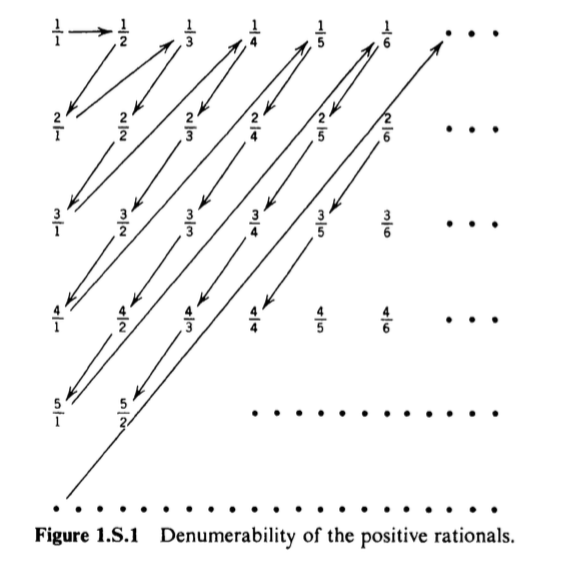
\includegraphics [scale=0.5] {denumerability.png} \end{center}
Basically, each row contains all the rational numbers with a particular numerator, and each column contains all the numbers with a particular denominator, arranged in strict increasing order.

Next, set up the sequence indicated by the arrows:
\[ \frac{1}{1} \ \ \ \ \ \frac{1}{2}, \frac{2}{1} \ \ \ \ \  \frac{1}{3}, \frac{2}{2}, \frac{3}{1} \ \ \ \ \ \frac{1}{4}, \frac{2}{3}, \frac{3}{2}, \frac{4}{1} \ \ \ \ \ \frac{1}{5}, \frac{2}{4}, \frac{3}{3}, \frac{4}{2}, \frac{5}{1} \ \ \ \ \ \frac{1}{6}, \frac{2}{5}, \frac{3}{4}, \frac{4}{3}, \frac{5}{2}, \frac{6}{1} \dots \]
Then remove all fractions that are duplicates because they are not in lowest terms.
\[ \frac{1}{1} \ \ \ \ \ \frac{1}{2}, \frac{2}{1} \ \ \ \ \  \frac{1}{3}, \frac{3}{1}\ \ \ \ \ \frac{1}{4}, \frac{2}{3}, \frac{3}{2}, \frac{4}{1} \ \ \ \ \ \frac{1}{5}, \frac{5}{1} \ \ \ \ \  \frac{1}{6}, \frac{2}{5}, \frac{3}{4}, \frac{4}{3}, \frac{5}{2}, \frac{6}{1} \dots \]

Finally, each $r$ in this sequence is assigned to a natural number (in the sequence $\mathbb{N}$), establishing the denumerability property.  $1/3$ is paired with $4$ and $3/1$ is paired with $5$, and so on.

Cantor showed that such a correspondence (which we just established for $\mathbb{Q}$), is impossible for $\mathbb{R}$.  The proof of this is is not hard, but we will skip it here.  You can check out the chapters on Georg Cantor in Dunham's \emph{Journey Through Genius}.

Thus, the rational numbers are said to be "countably infinite", while the real numbers are not countable.  (There is also a proof that the transcendental numbers are much more numerous than the non-transcendental ones).

So when we say that the set of numbers $r > 0$ has \emph{no least element}, our problem is two-fold.  We can pick a  rational member in the interval $(0,r)$, but subsequently, we can always find a smaller rational element.  

And once we get really close with the small rational element, there are infinitely more irrational than rational ones waiting beyond.  And yet, given any such very close irrational number, we can always find a smaller rational number, still larger than the bound.

I told you it was weird.

This property of the real numbers, that there is no closest number to any given number, accounts for virtually all of the theoretical difficulties in calculus which are solved by the use of limits and the apparatus of $\delta$ and $\epsilon$ or alternatively, neighborhoods.  For more, see the chapter on Limits and Continuity in the addendum.

\end{document}